\documentclass{article}
\usepackage{amsfonts}
\usepackage{amsmath}
\usepackage{mathtools}
\usepackage{systeme}
\usepackage{polynom}
\usepackage{pgfplots}
\usepackage[shortlabels]{enumitem}
\usepackage[a4paper,margin=1in,footskip=0.25in]{geometry}
\everymath{\displaystyle}
\DeclarePairedDelimiter\ceil{\lceil}{\rceil}
\newcommand{\p}[1]{\frac{\partial}{\partial #1}}
\begin{document}
\begin{center}
\Large\textbf{Kontrolltöö}\\
\small{Joosep Näks}
\end{center}
\textbf{2. Lahendus:}\\
Et saada esialgne punktid esialgses reeperis, on vaja pöörata punkte $-30^\circ$ võrra. Saan baasiteisenduse maatriksiks: 
\begin{gather*}
\begin{aligned}
X=
\begin{pmatrix}
\cos -30^\circ && -\sin -30^\circ\\
\sin -30^\circ && \cos -30^\circ\\
\end{pmatrix}=
\begin{pmatrix}
\frac{\sqrt{3}}2 && \frac12\\
-\frac12 && \frac{\sqrt{3}}2\\
\end{pmatrix}
\end{aligned}
\end{gather*}
Seega saan esialgsed punktid:
\begin{gather*}
\begin{aligned}
A=XA'&=\begin{pmatrix}\frac12-\sqrt{3}\\1+\frac{\sqrt{3}}{2}\end{pmatrix}\\
B=XB'&=\begin{pmatrix}2\sqrt{3}\\0\end{pmatrix}\\
C=XC'&=\begin{pmatrix}\frac12\\\frac{\sqrt{3}}2\end{pmatrix}\\
D=XD'&=\begin{pmatrix}0\\0\end{pmatrix}\\
\end{aligned}
\end{gather*}
\pagebreak\\
\textbf{3. Lahendus:}\\
Leian kõigepealt pikema pooltelje. Eksentrilisuse definitsiooni põhjal kehtib $e=\frac{c}{a}$, kus $e$ on eksentrilisus, $c$ fokaalpunkti kaugus keskpunktist ning $a$ pikema pooltelje pikkus. Kuna iga ellipsi punkti kauguste fokaalpunktidest summa on $2a$, peab lühema pooltelje kaugem ots olema kummastki fokaalpunktist $a$ kaugusel (kuna tekib võrdhaarne kolmnurk). Seega saab tekkinud võrdkülgsest kolmnurgast ellipsi keskpunkti, fokaalpunkti ja lühema pooltelje tipu vahel võrrandi $b^2+c^2=a^2$. Siia sisse asendades eksentrilisuse võrrandi, saab leida pikema pooltelje: $a=\frac{b}{\sqrt{1-e^2}}=\frac4{\sqrt{1-\frac1{2^2}}}=\frac8{\sqrt3}$.\\
Seega on ellipsi kanooniline võrrand $$\frac{x^2}{\frac{64}{3}}+\frac{y^2}{16}=1$$
Skitseeritud ellips:\\
\begin{figure}[htbp]
\centerline{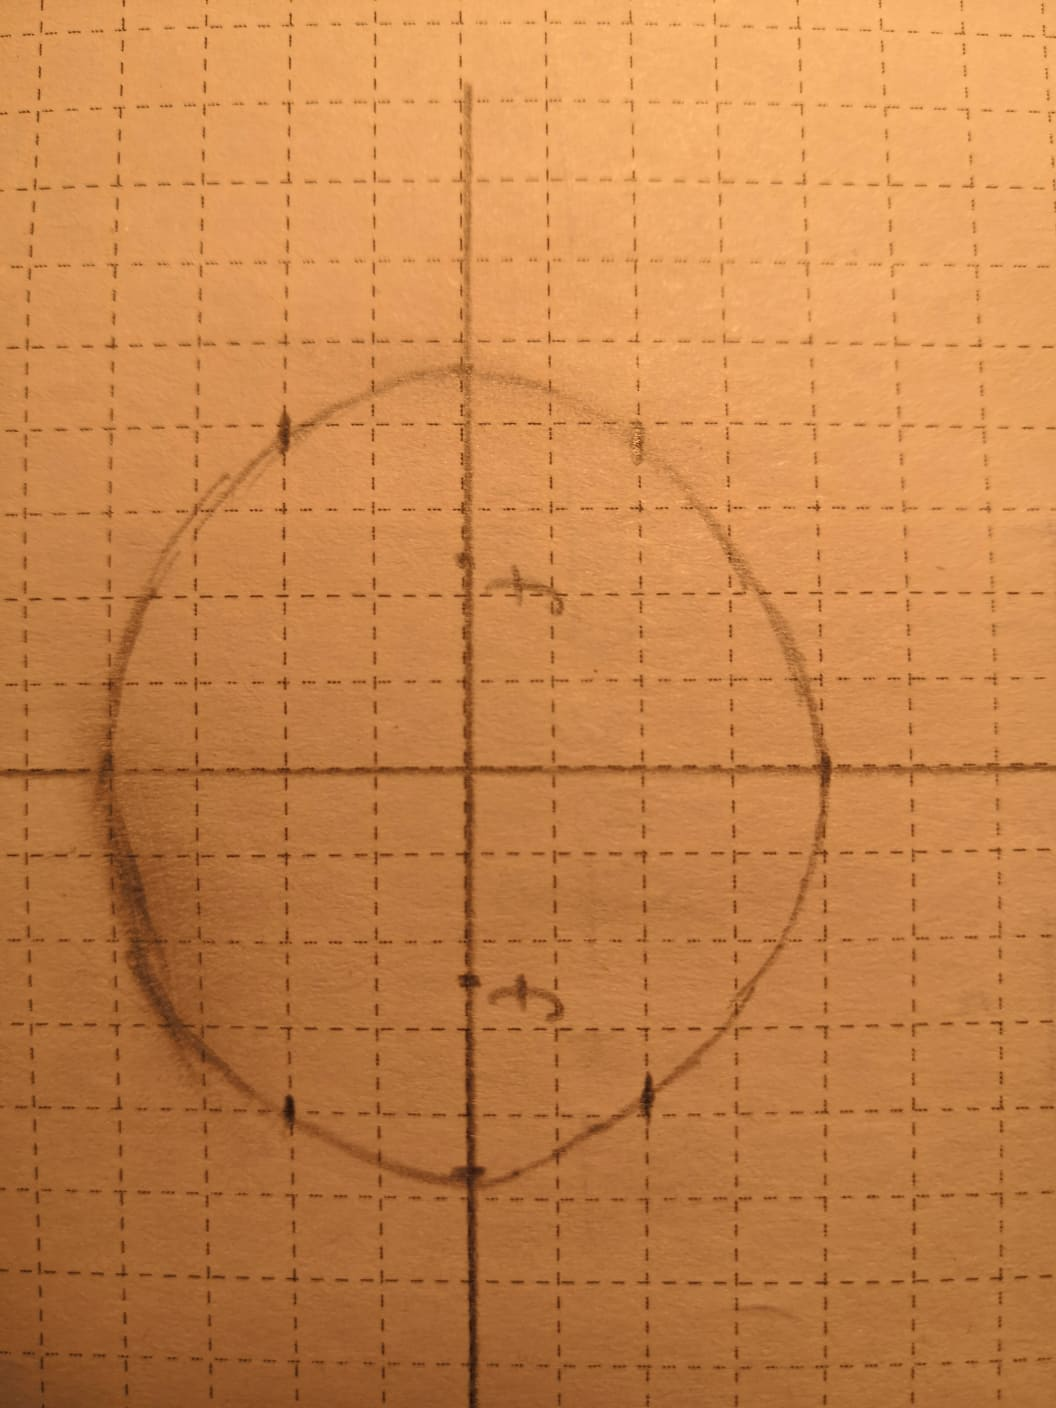
\includegraphics[scale=0.2,angle=90]{ellips.jpg}}
\end{figure}\\
Fookuspunktid asuvad punktides $(c,0)$ ja $(-c,0)$ ehk $(\frac{16}3,0)$ ja $(-\frac{16}3,0)$
\pagebreak\\
\textbf{4. Lahendus:}\\
Võrrandit teisendades saan võrrandi: $$\frac{x^2}{\frac{29}{20}}-\frac{(y-\frac12)^2}{\frac{29}{12}}=1$$ Siit on näha, et tema keskpunkt on $\left(0,\frac12\right)$, poolteljed $a=\frac{29}{20}$ ja $b=\frac{29}{12}$, asümptoodid $y=\sqrt{\frac{5}{3}}x+\frac12$ ja $y=-\sqrt{\frac{5}{3}}x+\frac12$. Fookuste kaugus keskpunktist on $c=\sqrt{a^2+b^2}=\sqrt{\frac{58}{15}}$ ehk eksentrilisus on $e=\frac{c}{a}=\sqrt{\frac83}$ ning fookused asuvad punktides $F_1\left(\sqrt{\frac{58}{15}},\frac12\right)$ ja $F_2\left(-\sqrt{\frac{58}{15}},\frac12\right)$. Fokaalparameetriks saan $q=\frac{b^2}{a}=\frac{\sqrt{145}}{6}$.\\
\pagebreak\\
\textbf{5. Lahendus:}\\
Teen kõigepealt nihke $(-1,-2)$, et saada keskpunktiks $(1,2)$: $A(1,2)\rightarrow A'(0,0)$, $B(-2,4)\rightarrow B'(-3,2)$. Seejärel pööran baasi $30^\circ$ võrra maatriksiga 
\begin{gather*}
\begin{aligned}
X=
\begin{pmatrix}
\cos 30^\circ && -\sin 30^\circ\\
\sin 30^\circ && \cos 30^\circ\\
\end{pmatrix}=
\begin{pmatrix}
\frac{\sqrt{3}}2 && -\frac12\\
\frac12 && \frac{\sqrt{3}}2\\
\end{pmatrix}
\end{aligned}
\end{gather*}
Saan punktid $A''=XA'=(0,0)$, $B''=XB'=\left(-\frac{3\sqrt{3}}{2}-1, \sqrt3-\frac12\right)$.
Teen vahetuse polaarkoordinaatidesse: $r_A=\sqrt{0^2+0^2}=0$, $\theta_A=\arctan\left(\frac{0}{0}\right)=0$, $r_B=\sqrt{\left(-\frac{3\sqrt{3}}{2}-1\right)^2+\left(\sqrt3-\frac12\right)^2}=\sqrt{11+2\sqrt{3}}$, $\theta_B=\arctan\left(\frac{-\frac{3\sqrt{3}}{2}-1}{\sqrt3-\frac12}\right)$.
\end{document}